\documentclass[]{ctexbook}
\usepackage{lmodern}
\usepackage{amssymb,amsmath}
\usepackage{ifxetex,ifluatex}
\usepackage{fixltx2e} % provides \textsubscript
\ifnum 0\ifxetex 1\fi\ifluatex 1\fi=0 % if pdftex
  \usepackage[T1]{fontenc}
  \usepackage[utf8]{inputenc}
\else % if luatex or xelatex
  \ifxetex
    \usepackage{xltxtra,xunicode}
  \else
    \usepackage{fontspec}
  \fi
  \defaultfontfeatures{Ligatures=TeX,Scale=MatchLowercase}
\fi
% use upquote if available, for straight quotes in verbatim environments
\IfFileExists{upquote.sty}{\usepackage{upquote}}{}
% use microtype if available
\IfFileExists{microtype.sty}{%
\usepackage{microtype}
\UseMicrotypeSet[protrusion]{basicmath} % disable protrusion for tt fonts
}{}
\usepackage[b5paper,tmargin=2.5cm,bmargin=2.5cm,lmargin=3.5cm,rmargin=2.5cm]{geometry}
\usepackage[unicode=true]{hyperref}
\PassOptionsToPackage{usenames,dvipsnames}{color} % color is loaded by hyperref
\hypersetup{
            pdftitle={Face lab book},
            pdfauthor={Face lab},
            colorlinks=true,
            linkcolor=Maroon,
            citecolor=Blue,
            urlcolor=Blue,
            breaklinks=true}
\urlstyle{same}  % don't use monospace font for urls
\usepackage{natbib}
\bibliographystyle{apalike}
\usepackage{longtable,booktabs}
% Fix footnotes in tables (requires footnote package)
\IfFileExists{footnote.sty}{\usepackage{footnote}\makesavenoteenv{long table}}{}
\usepackage{graphicx,grffile}
\makeatletter
\def\maxwidth{\ifdim\Gin@nat@width>\linewidth\linewidth\else\Gin@nat@width\fi}
\def\maxheight{\ifdim\Gin@nat@height>\textheight\textheight\else\Gin@nat@height\fi}
\makeatother
% Scale images if necessary, so that they will not overflow the page
% margins by default, and it is still possible to overwrite the defaults
% using explicit options in \includegraphics[width, height, ...]{}
\setkeys{Gin}{width=\maxwidth,height=\maxheight,keepaspectratio}
\IfFileExists{parskip.sty}{%
\usepackage{parskip}
}{% else
\setlength{\parindent}{0pt}
\setlength{\parskip}{6pt plus 2pt minus 1pt}
}
\setlength{\emergencystretch}{3em}  % prevent overfull lines
\providecommand{\tightlist}{%
  \setlength{\itemsep}{0pt}\setlength{\parskip}{0pt}}
\setcounter{secnumdepth}{5}
% Redefines (sub)paragraphs to behave more like sections
\ifx\paragraph\undefined\else
\let\oldparagraph\paragraph
\renewcommand{\paragraph}[1]{\oldparagraph{#1}\mbox{}}
\fi
\ifx\subparagraph\undefined\else
\let\oldsubparagraph\subparagraph
\renewcommand{\subparagraph}[1]{\oldsubparagraph{#1}\mbox{}}
\fi

% set default figure placement to htbp
\makeatletter
\def\fps@figure{htbp}
\makeatother

\usepackage{booktabs}
\usepackage{longtable}

\usepackage{framed,color}
\definecolor{shadecolor}{RGB}{248,248,248}

\renewcommand{\textfraction}{0.05}
\renewcommand{\topfraction}{0.8}
\renewcommand{\bottomfraction}{0.8}
\renewcommand{\floatpagefraction}{0.75}

\let\oldhref\href
\renewcommand{\href}[2]{#2\footnote{\url{#1}}}

\makeatletter
\newenvironment{kframe}{%
\medskip{}
\setlength{\fboxsep}{.8em}
 \def\at@end@of@kframe{}%
 \ifinner\ifhmode%
  \def\at@end@of@kframe{\end{minipage}}%
  \begin{minipage}{\columnwidth}%
 \fi\fi%
 \def\FrameCommand##1{\hskip\@totalleftmargin \hskip-\fboxsep
 \colorbox{shadecolor}{##1}\hskip-\fboxsep
     % There is no \\@totalrightmargin, so:
     \hskip-\linewidth \hskip-\@totalleftmargin \hskip\columnwidth}%
 \MakeFramed {\advance\hsize-\width
   \@totalleftmargin\z@ \linewidth\hsize
   \@setminipage}}%
 {\par\unskip\endMakeFramed%
 \at@end@of@kframe}
\makeatother

\makeatletter
\@ifundefined{Shaded}{
}{\renewenvironment{Shaded}{\begin{kframe}}{\end{kframe}}}
\@ifpackageloaded{fancyvrb}{%
  % https://github.com/CTeX-org/ctex-kit/issues/331
  \RecustomVerbatimEnvironment{Highlighting}{Verbatim}{commandchars=\\\{\},formatcom=\xeCJKVerbAddon}%
}{}
\makeatother

\usepackage{makeidx}
\makeindex

\urlstyle{tt}

\usepackage{amsthm}
\makeatletter
\def\thm@space@setup{%
  \thm@preskip=8pt plus 2pt minus 4pt
  \thm@postskip=\thm@preskip
}
\makeatother

\frontmatter

\title{Face lab book}
\author{Face lab}
\date{2024-11-09}

\begin{document}
\maketitle


\thispagestyle{empty}

\begin{center}
献给……

\end{center}

\setlength{\abovedisplayskip}{-5pt}
\setlength{\abovedisplayshortskip}{-5pt}

{
\setcounter{tocdepth}{2}
\tableofcontents
}
\listoftables
\listoffigures
\chapter{简介}\label{ux7b80ux4ecb}

这是面孔实验室的实验手册,目前主要尝试介绍一些常用的软件或技术。

实验室目前常用的软件有:

\begin{itemize}
\tightlist
\item
  Chapter \ref{jamovi}: Jamovi\\
\item
  Chapter \ref{zotero}: Zotero
\end{itemize}

\mainmatter

\part{统计软件}\label{part-ux7edfux8ba1ux8f6fux4ef6}

\chapter{Jamovi}\label{jamovi}

汇总:沈佳欣、张宇杰\\
更新于:2024-11-07

\section{方差分析}\label{ux65b9ux5deeux5206ux6790}

导入数据后,依次点击``分析''\,``方差分析''选项,然后在弹出的选项栏中选择适当的方差分析方法。前五个为参数检验方法,后两个为非参数检验方法,它们分别对应统计课本中的克-瓦氏单向方差分析和弗里德曼两因素等级方差分析。

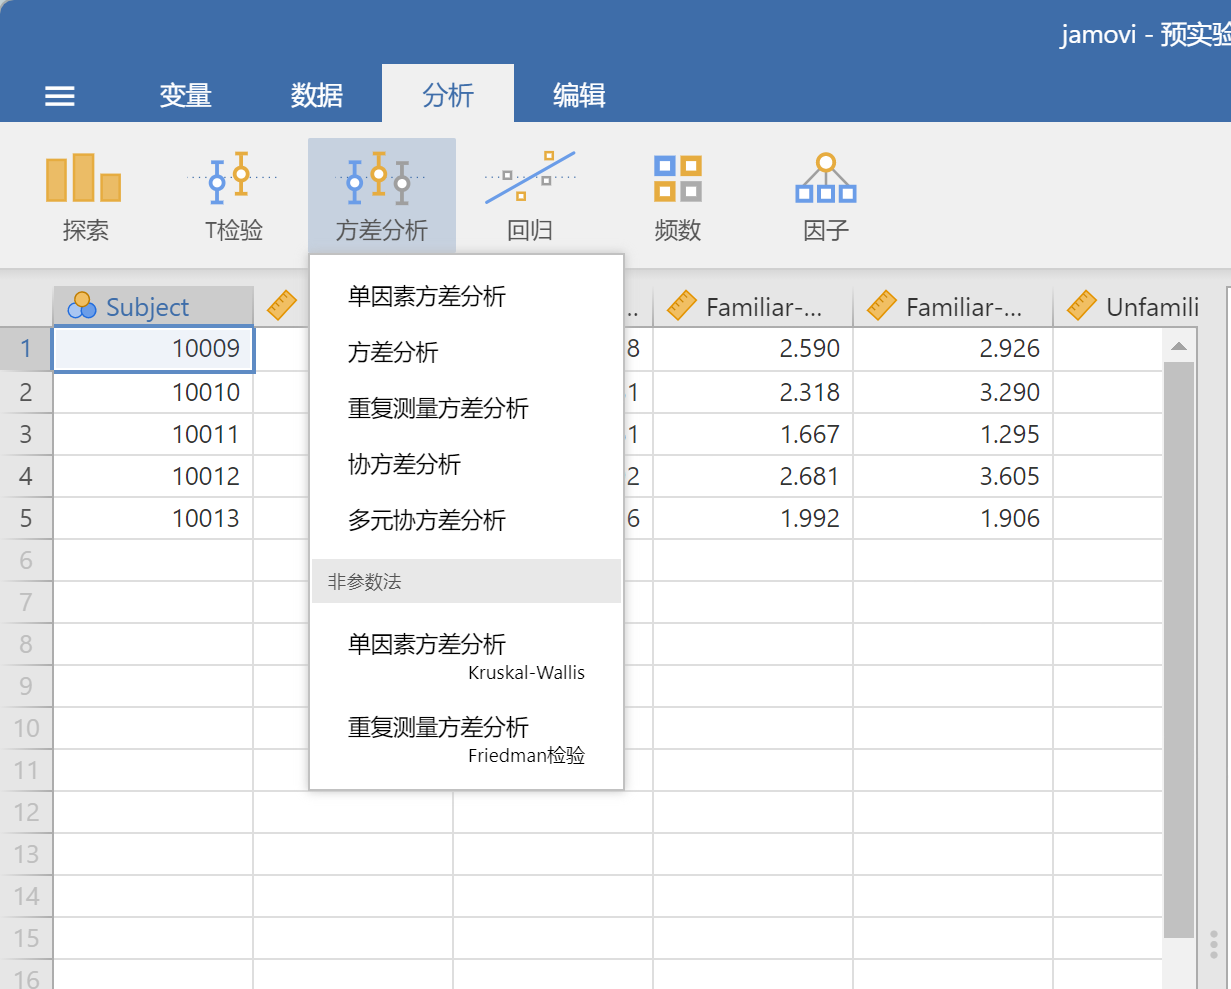
\includegraphics{img/jamovi/anova.png}

此次以重复测量方差分析为例。在下图左侧的界面里,左侧是我们数据的名称,右侧的``重复测量因子''是指在研究中设置的``被试内自变量''。在本例中,我们有三个``被试内自变量'',每个自变量都有两个水平。例如我们将``重复测量因子1''定义为Familiar,它包括``familiar''和``unfamiliar''两个水平。

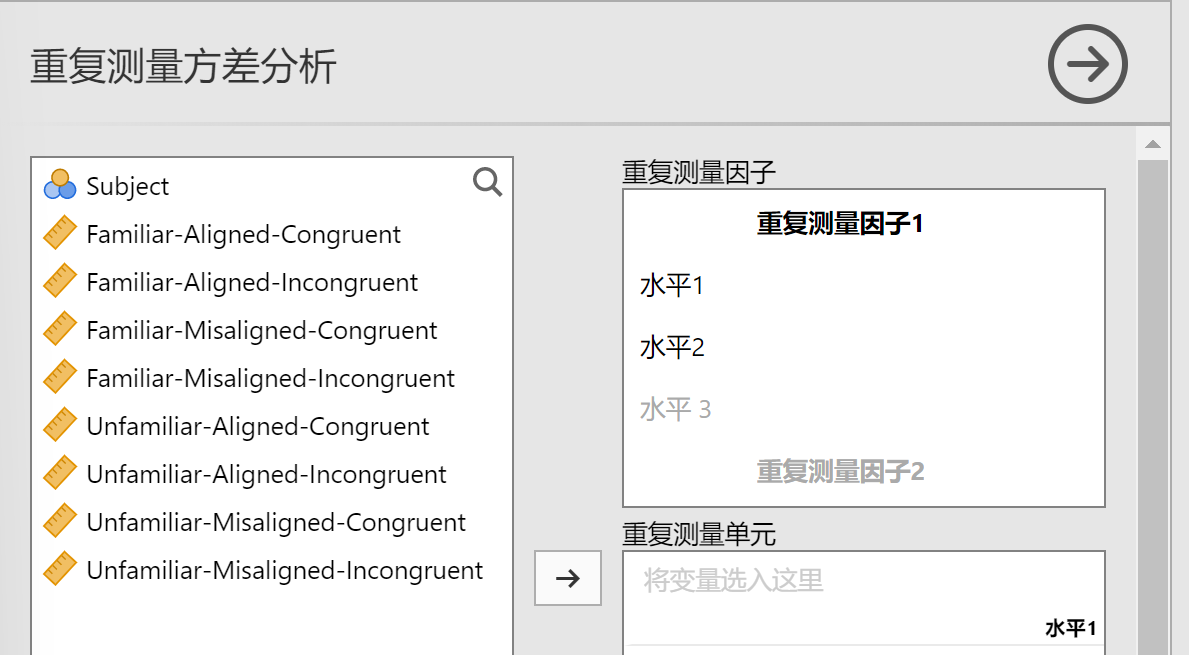
\includegraphics{img/jamovi/rmanova-factor.png}\\
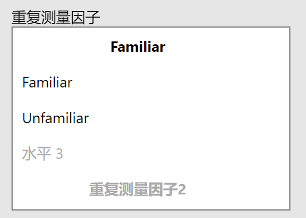
\includegraphics{img/jamovi/rmanova-factorlevels.png}

定义好重复测量因子后,``重复测量单元''中会出现各个自变量水平的组合,而``重复测量单元''也就是指研究中的各种实验条件。在本例中我们的实验是一个2 * 2 * 2的被试内设计,所以共有8种实验条件,我们需要做的是将数据拖入其对应的重复测量单元中。

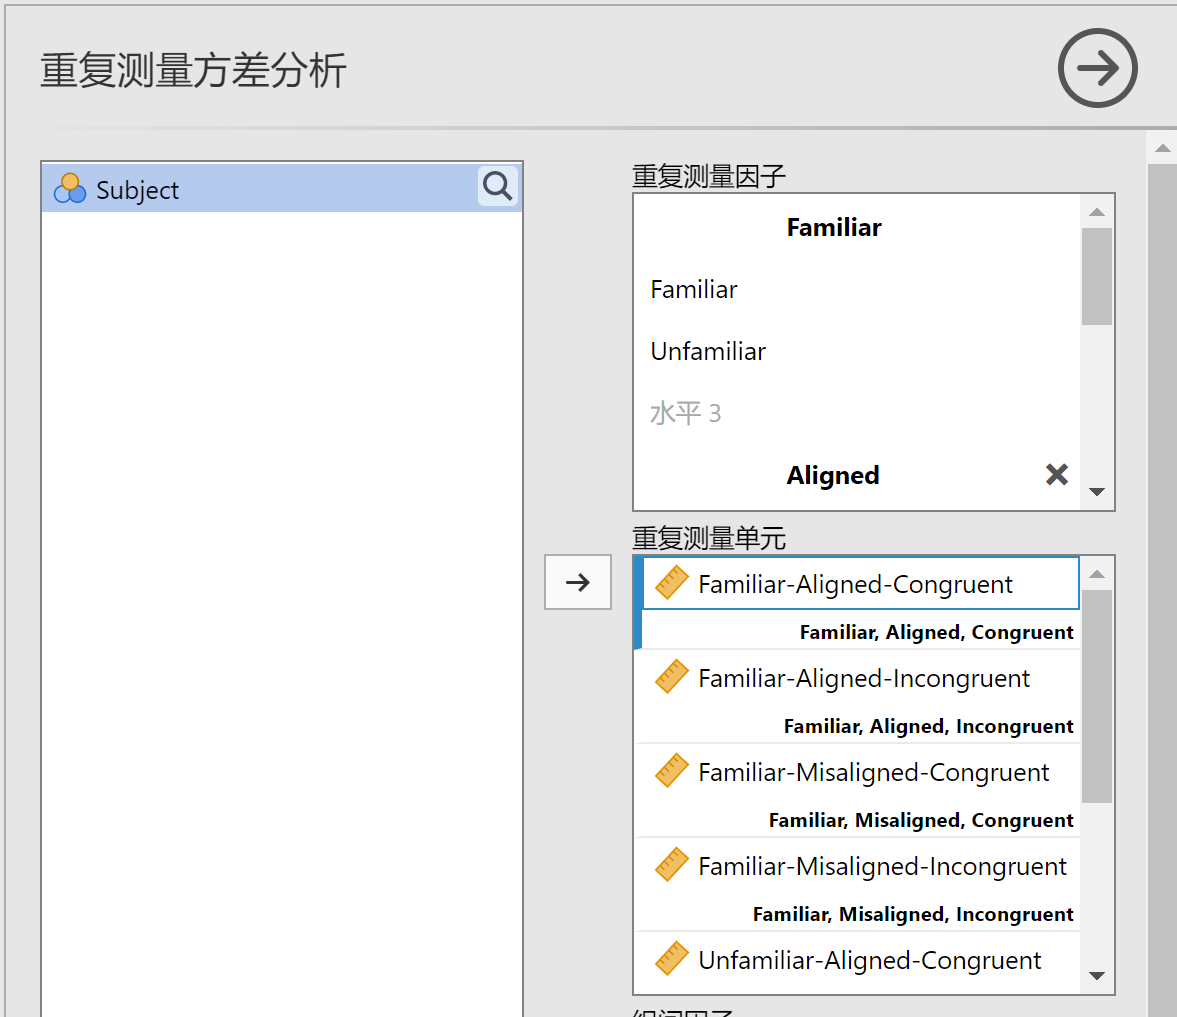
\includegraphics{img/jamovi/rmanova-factorlevels2.png}

接下来我们要选择效应量为``偏η²值'',以及确定因变量标签。本例中因变量标签为``d-prime''.

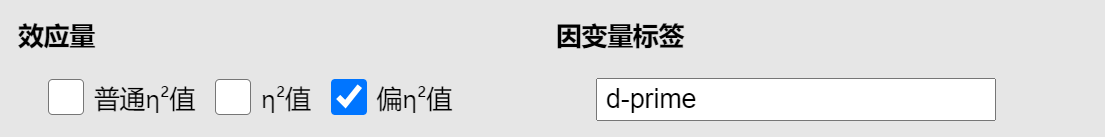
\includegraphics{img/jamovi/rmanova-dv.png}

下面的五个选项里,我们应当关注的主要是``适用条件判断''和``事后检验''。

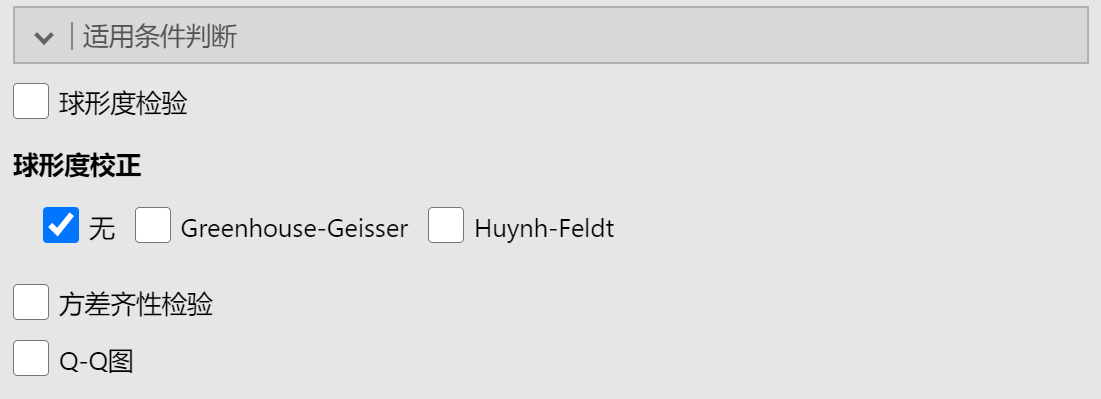
\includegraphics{img/jamovi/rmanova-sphericity.png}

对本专业来说,在这一栏中较为重要的是``方差齐性检验'',如果变量中涉及被试间变量,那么应当进行方差齐性检验。但由于本例中的变量都是被试内变量,所以无需进行方差齐性检验。其他几个选项可以根据研究所需进行选取。

所有设定完成后,jamovi会在右侧呈现数据分析结果。

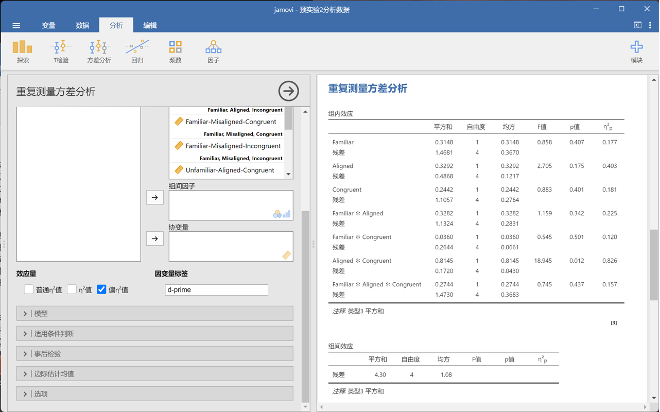
\includegraphics{img/jamovi/rmanova-result.png}

\section{简单效应分析}\label{ux7b80ux5355ux6548ux5e94ux5206ux6790}

这一部分承接上述重复测量方差分析。在本例中,当我们在jamovi中确定好了``重复测量因子''即``被试内变量''和``重复测量单元''即``实验条件''后,我们可以看到右侧的结果栏中就可以呈现统计结果,如果某两个或几个变量之间存在显著的交互作用,那么我们应当进行事后检验,以确定一个变量在与它有交互作用的另一个变量的哪些水平上显著,哪些水平上不显著。我们需要选择下列五个选项中的``事后检验''。

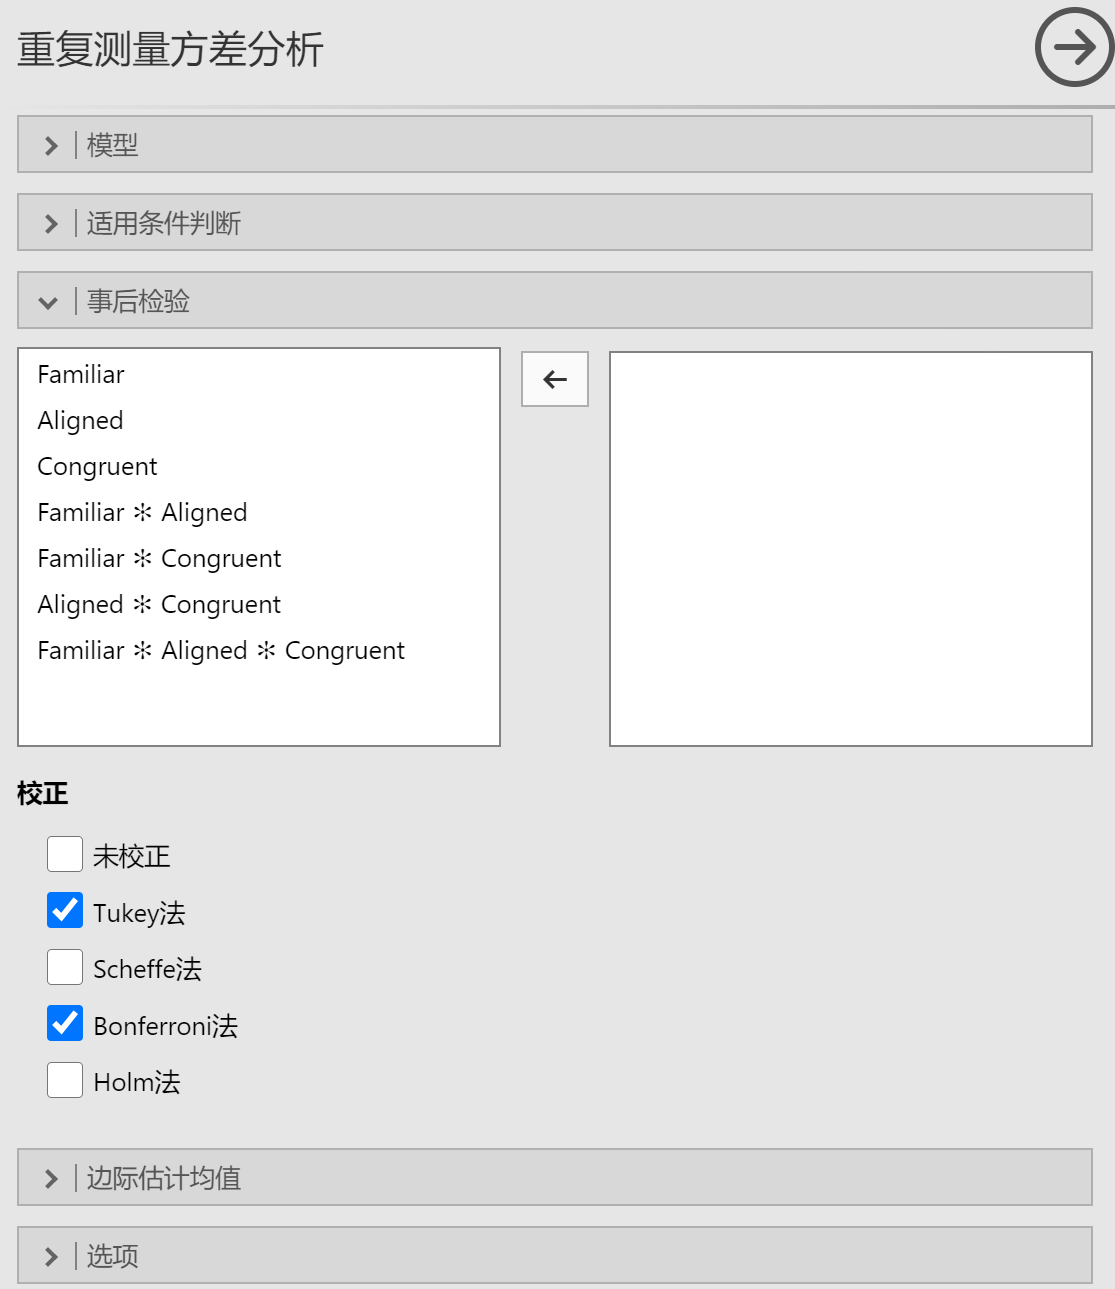
\includegraphics{img/jamovi/rmanova-posthoc.png}

选择需要进行事后检验的交互变量,并按照需要选择恰当的校正方法。

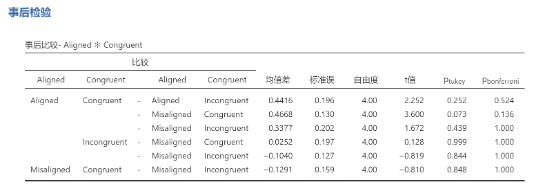
\includegraphics{img/jamovi/rmanova-posthoc-results.png}

右侧生成的结果的最右边两列就是jamovi按照我们选择的Tukey法和Bonferron法计算出的统计值。

\section{t检验}\label{tux68c0ux9a8c}

\begin{itemize}
\tightlist
\item
  首先,导入数据
\item
  其次,点击选项栏的分析,选择对应的t检验
\end{itemize}

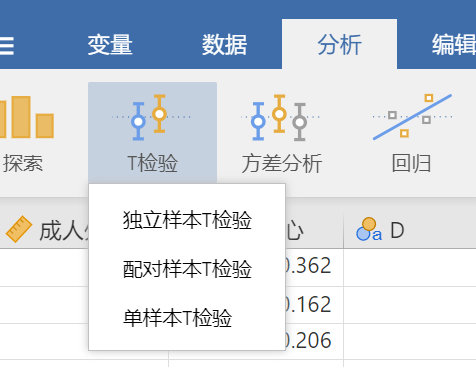
\includegraphics{img/jamovi/ttest.png}

\begin{itemize}
\tightlist
\item
  接着,选择要分析的变量
\end{itemize}

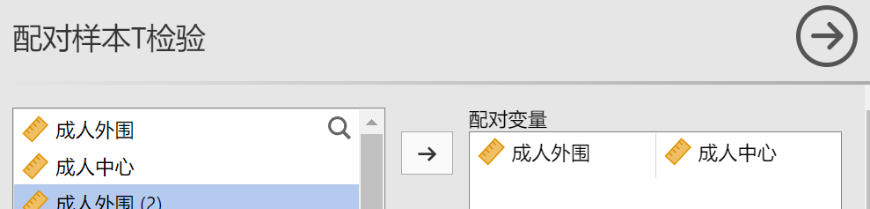
\includegraphics{img/jamovi/ttest-compare.png}

\begin{itemize}
\tightlist
\item
  然后,可以按需勾选,描述就是分析数据的均值、标准差、标准误等描述性数据;描述图就是生成图表
\end{itemize}

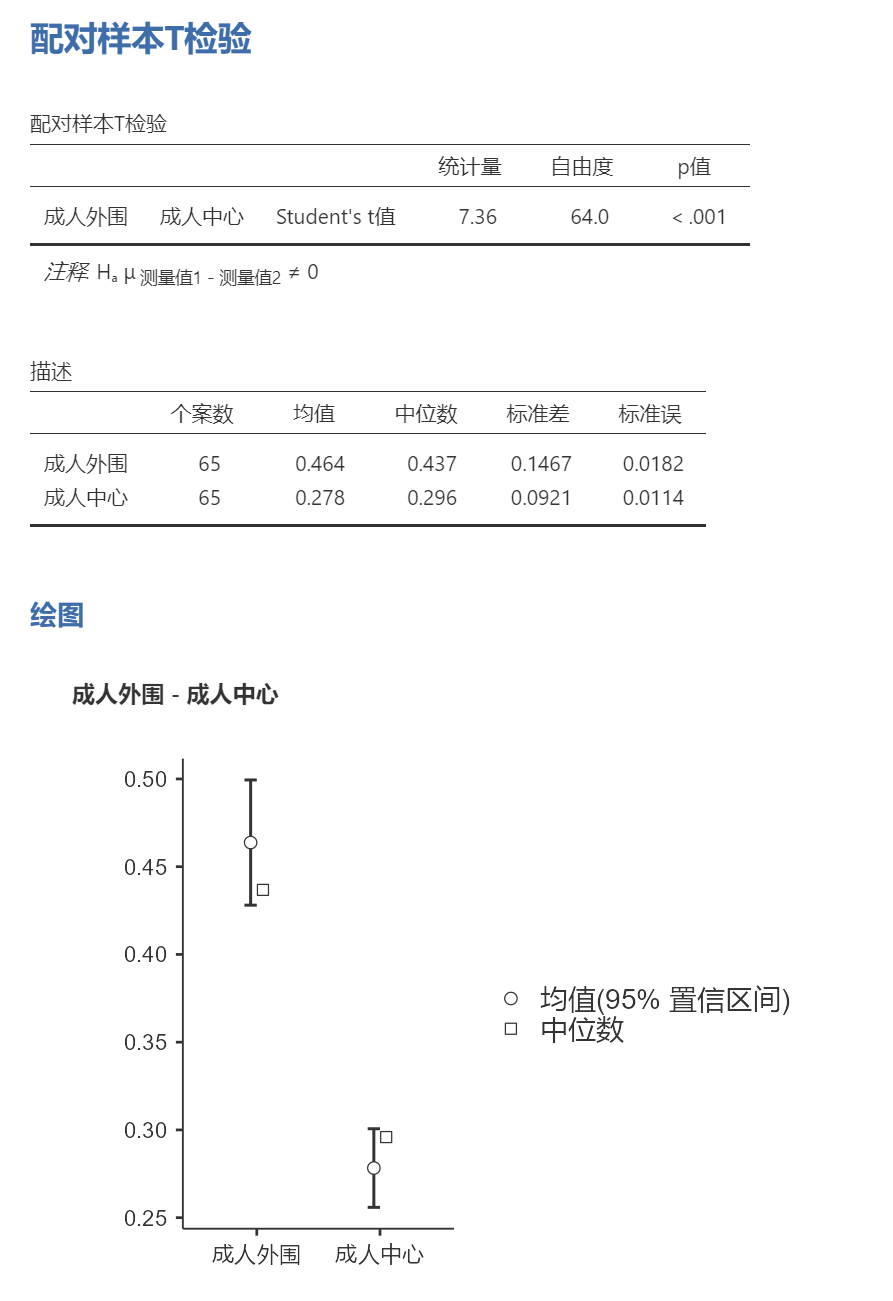
\includegraphics{img/jamovi/ttest-results.png}

\section{额外模块推荐}\label{ux989dux5916ux6a21ux5757ux63a8ux8350}

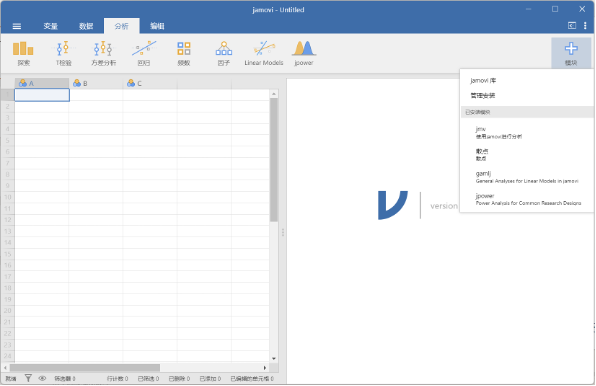
\includegraphics{img/jamovi/modules.png}\\
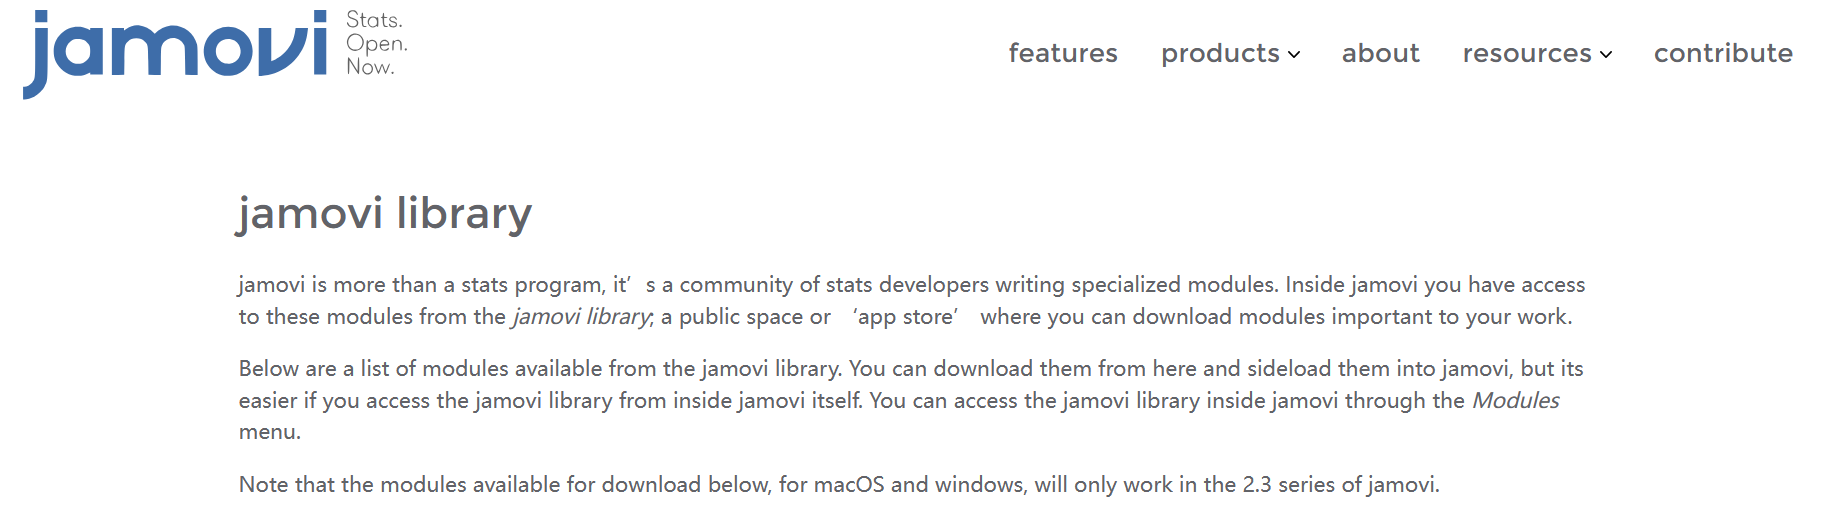
\includegraphics{img/jamovi/modules-library.png}

可以通过jamovi官网下载自己所需要的库。这是网址:\url{https://www.jamovi.org/library.html}

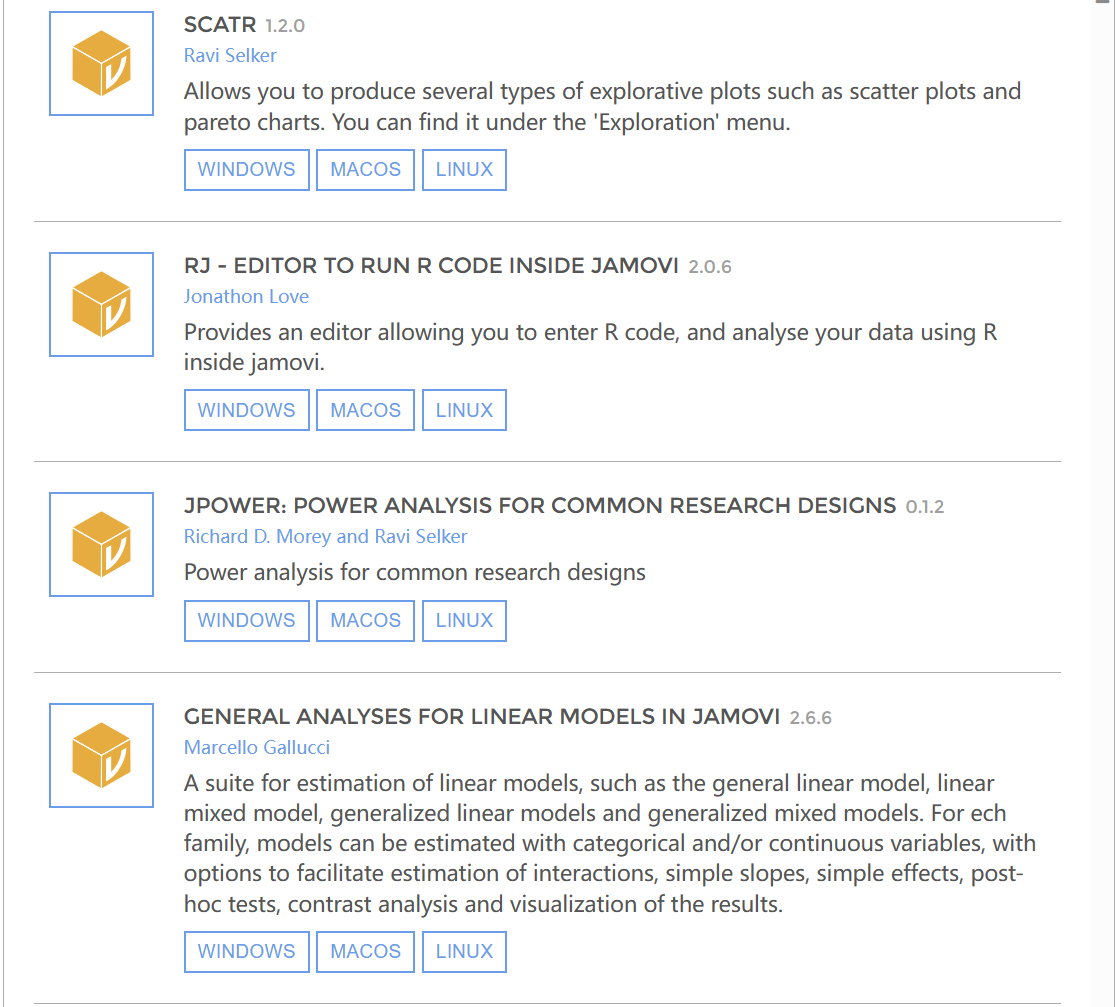
\includegraphics{img/jamovi/modules1.png}\\
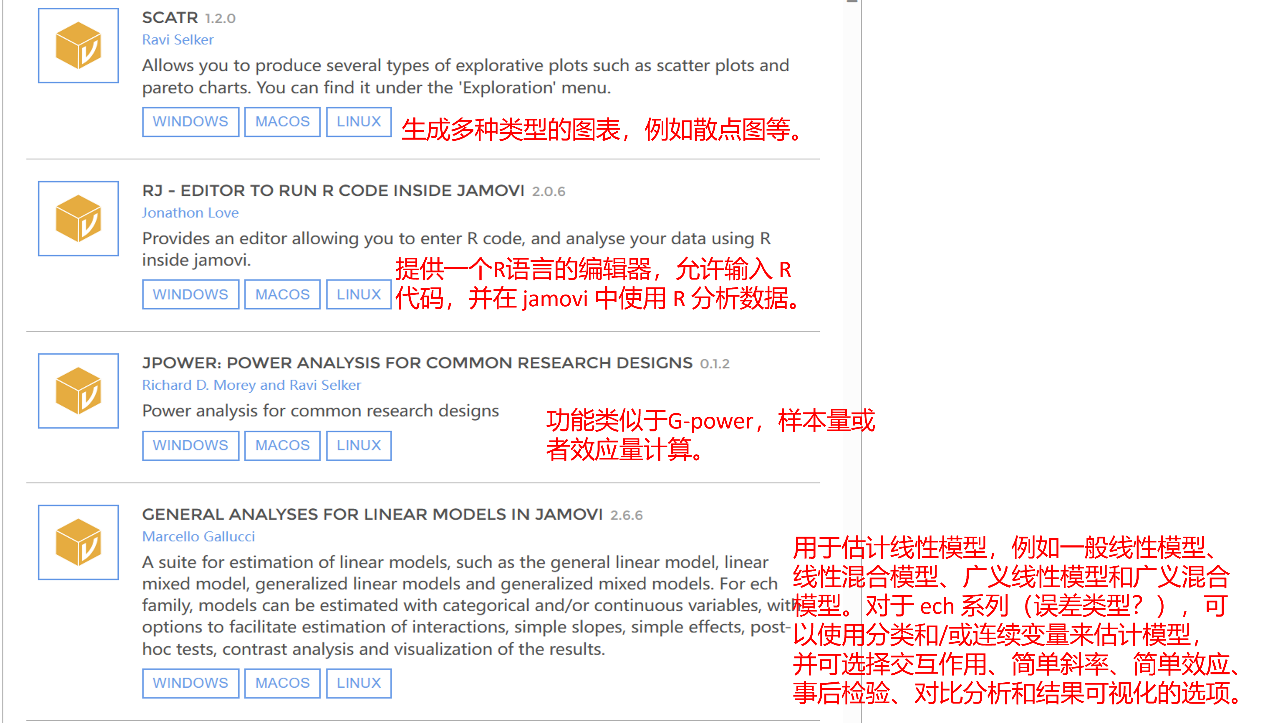
\includegraphics{img/jamovi/modules2.png}\\
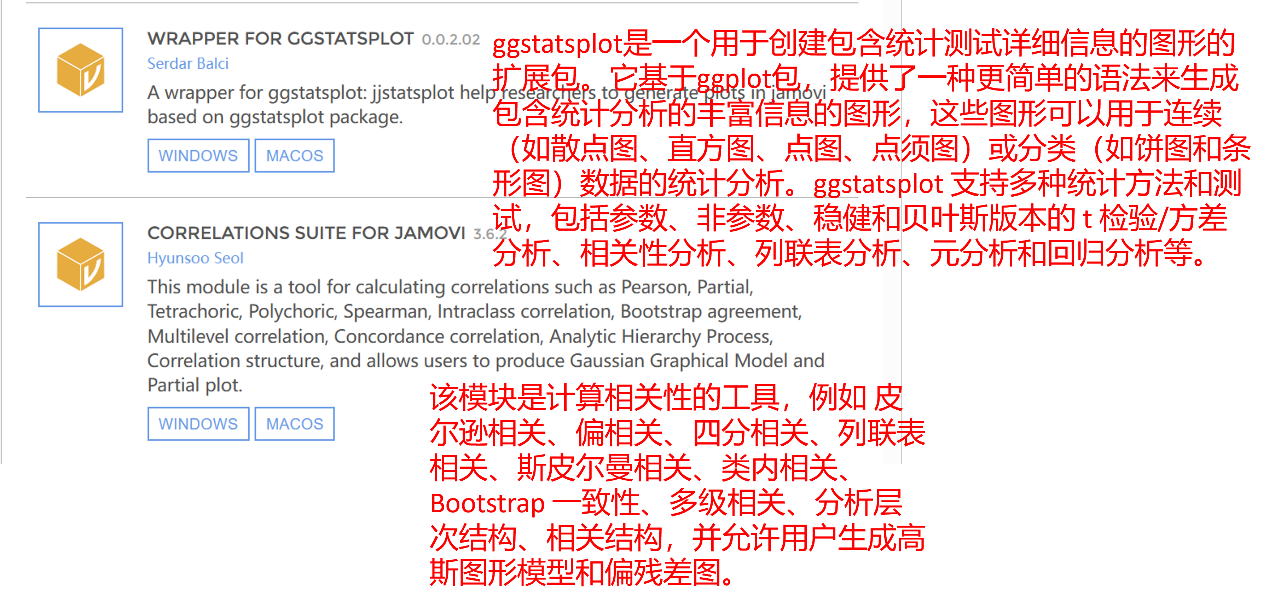
\includegraphics{img/jamovi/modules3.png}\\
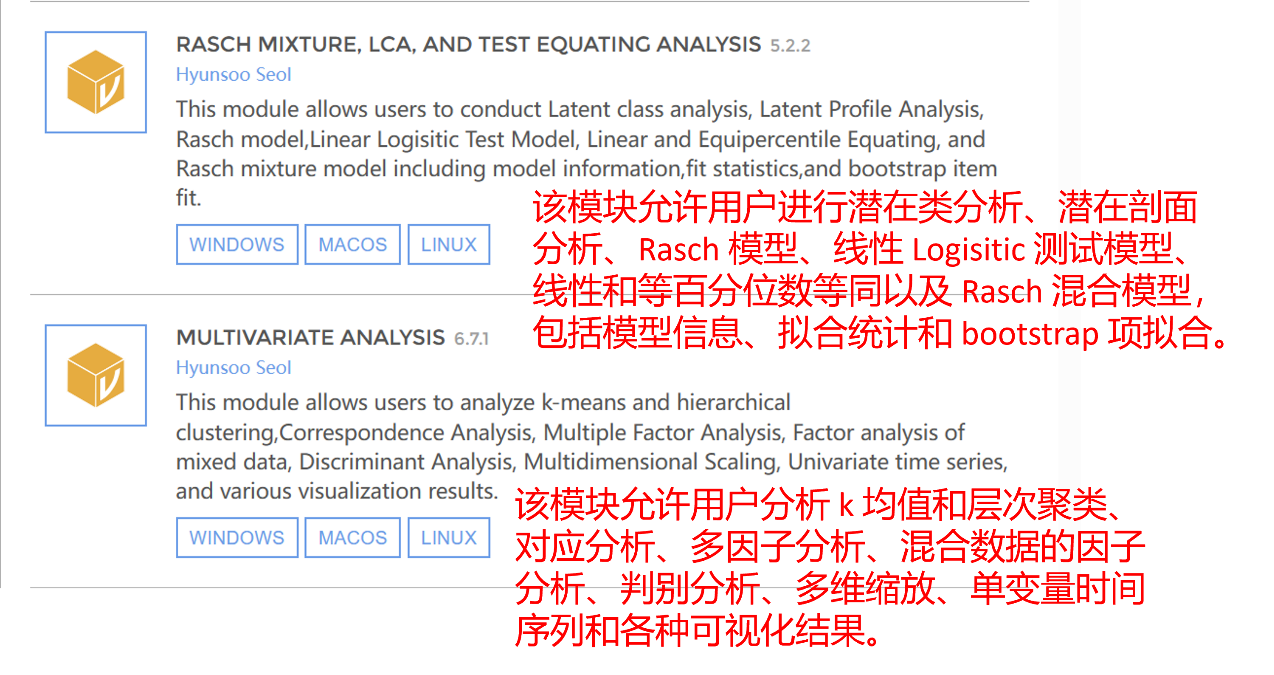
\includegraphics{img/jamovi/modules4.png}

\chapter{R语言}\label{r}

\section{预处理数据}\label{r-prepro}

汇总:
更新于:

\section{重复测量方差分析}\label{r-rm-anova}

汇总:
更新于:

\section{数据可视化}\label{r-plot}

汇总:
更新于:

\part{科研工具}\label{part-ux79d1ux7814ux5de5ux5177}

\chapter{Zotero}\label{zotero}

汇总:郭沫然\\
更新于:

\part{实验材料和公开数据}\label{part-ux5b9eux9a8cux6750ux6599ux548cux516cux5f00ux6570ux636e}

\chapter{实验材料}\label{materials}

汇总:\\
更新于:

\section{Chicago Face Database (芝加哥面孔数据库)}\label{chicago-face-database-ux829dux52a0ux54e5ux9762ux5b54ux6570ux636eux5e93}

\href{https://www.chicagofaces.org/}{Chicago Face Database}

Ma, D. S., Correll, J., \& Wittenbrink, B. (2015). The Chicago face database: A free stimulus set of faces and norming data. \emph{Behavior Research Methods}, 47(4), 1122--1135. \url{https://doi.org/10.3758/s13428-014-0532-5}

Ma, D. S., Kantner, J., \& Wittenbrink, B. (2021). Chicago Face Database: Multiracial expansion. \emph{Behavior Research Methods}, 53(3), 1289--1300. \url{https://doi.org/10.3758/s13428-020-01482-5}

\chapter{公开数据库}\label{opendata}

汇总:\\
更新于:

\section{磁共振(fMRI)}\label{ux78c1ux5171ux632ffmri}

\section{脑电(EEG)}\label{ux8111ux7535eeg}

\section{行为}\label{ux884cux4e3a}

\cleardoublepage

\appendix \addcontentsline{toc}{chapter}{\appendixname}


\chapter{如何为本手册作出贡献}\label{ux5982ux4f55ux4e3aux672cux624bux518cux4f5cux51faux8d21ux732e}

\bibliography{references.bib,packages.bib}

\backmatter
\printindex

\end{document}
